Als mächtigste Weltmacht beeinflussen die Vereinigten Staaten nahezu jeden Teil des Globus. Mitunter deshalb und aufgrund der enormen Präsenz in den Medien sowie des Einflusses auf diese fallen Diskrepanzen in der Bevölkerung schneller auf als in anderen Ländern. Aufgrund dieser Stellung wirkt sich die dortige Sentimentalität somit auch auf das Leben in anderen Ländern aus. Der Kapitolsanschlag sowie die Black Lives Matter Proteste der letzten Jahre sind ein Zeichen für die zunehmende Polarität und Unzufriedenheit in der Bevölkerung, wie sich auch in folgender Grafik erkennen lässt \label{polPolar} \citelit{politicalPolarization}.

\begin{figure}[ht]
	\centering
	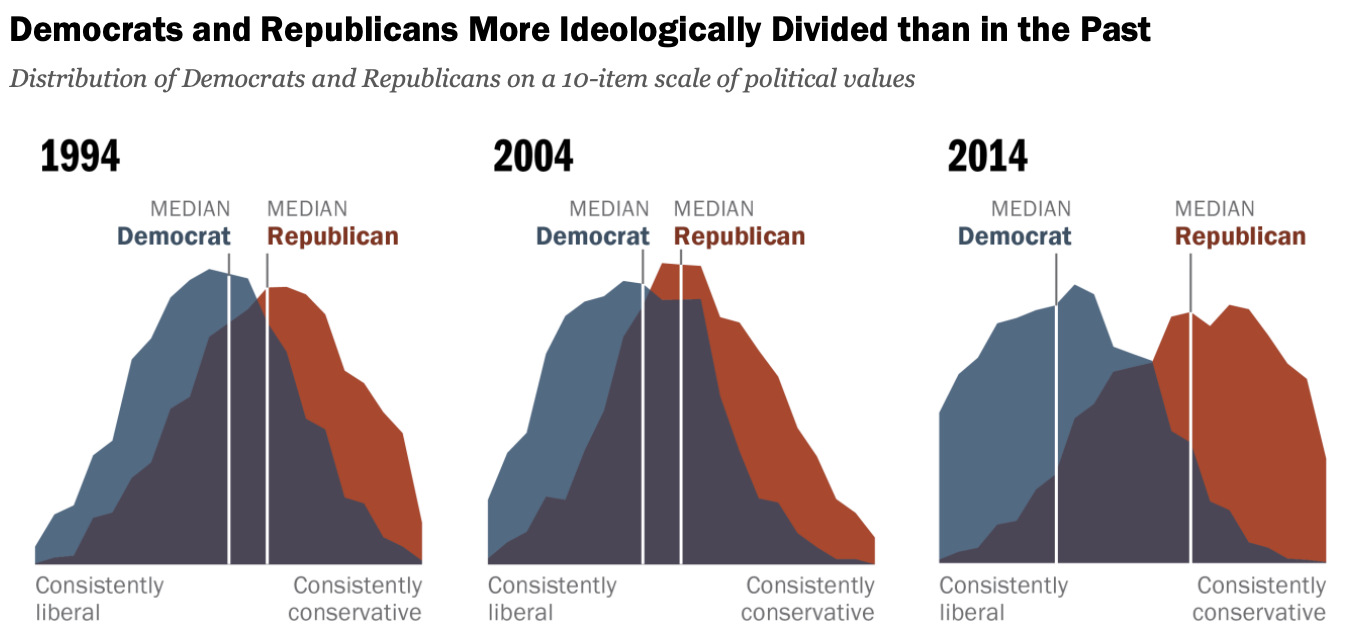
\includegraphics[width=1\textwidth]{images/Kapitel1/PoliticalPolarization}
	\caption{\label{fig:polPolar}Entwicklung der Polarität politisch engagierter Amerikaner.}{Basierend auf 10 politischen Metriken werden Demokraten (blau) und Republikaner (rot) hier verglichen. Wie zu erkennen bewegen sich die zu Beginn teils noch überlappenden Ideologien in den letzten 10 Jahren auseinander \protect\citelit{politicalPolarization}.}
\end{figure}

Aufgabe dieser Arbeit ist es nicht, sich mit den komplexen und vielschichtigen Hintergründen für diese Entwicklung auseinanderzusetzen. Vielmehr wird hiermit versucht, eben diese Polarität in den oberen Reihen der amerikanischen Politik genauer zu analysieren.

Unsere Zielsetzung bestand darin, mit den Tweets der letzten 12 Jahre von 420 Politikern des Repräsentantenhauses eine Sentimentalitätsanalyse durchzuführen. Dabei handelt es sich um ein Mittel der natürlichen Sprachverarbeitung, bei dem die Ansicht beziehungsweise Gefühlslage eines Textes quantifiziert wird.